\documentclass[xcolor={dvipsnames},pdf, hyperref={colorlinks=true, citecolor=ForestGreen, linkcolor=BlueViolet, urlcolor=Magenta}]{beamer}
\usetheme{Frankfurt}  
\usecolortheme{whale}
\usepackage{tikz} 
\usepackage{graphicx}
\usepackage{dsfont}
\usepackage{hyperref}
\usepackage{alltt}
\usepackage{enumerate}
\usepackage{amsthm}
\theoremstyle{definition}
\newtheorem{exmp}{Example}[section]
\usepackage{verbatim}               % useful for \begin{comment} and \end{comment}
\usepackage{eurosym}                % used for euro symbol
\usepackage{caption} 
\usepackage{graphicx}
\usepackage{adjustbox}
\graphicspath{{Figures/}}
\usepackage{subcaption}
\usepackage{color}
\usepackage{float}
\usepackage{amssymb}
\usepackage{MnSymbol,wasysym}
\usepackage{sgamevar}
\usepackage{remreset}% tiny package containing just the \@removefromreset command
\makeatletter
\@removefromreset{subsection}{section}
\makeatother
\setcounter{subsection}{1}



\newcommand{\defn}[1]{\textbf{#1}}


%Instructor version
\newcommand{\blank}[0]{}
\newcommand{\ddp}[1]{{\textcolor{ForestGreen}{#1}}} 
\newcommand{\dd}[1]{{\underline{\textcolor{ForestGreen}{#1}}}}

%Student version
%\newcommand{\blank}[0]{\vspace{2em}}
%\newcommand{\dd}[1]{\underline{\hspace{3cm}}} 
%\newcommand{\ddp}[1]{}

\addtobeamertemplate{navigation symbols}{}{%
	\usebeamerfont{footline}%
	\usebeamercolor[fg]{footline}%
	\hspace{1em}%
	\insertframenumber/\inserttotalframenumber
}

\section{Monetary Policy}

%% preamble
\title{Monetary and Fiscal Policy}
\author{David A. D\'iaz}
\date{}

\AtBeginSection[] %Section links on slides

\begin{document} 
	
	\begin{frame}
		
		\titlepage
		
	\end{frame}

\begin{frame}{Monetary Policy \& Fiscal Policy}
\begin{itemize}
	\item We saw that shifts in aggregate demand and aggregate supply can lead to short run periods of expansion and recession, as well as affect both the short run and long run inflation rate in an economy.
	\item Given this, is there anything the Federal reserve or the federal government can do that mitigates such fluctuations?
\end{itemize}
\end{frame}

\begin{frame}{Monetary Policy}
\begin{itemize}
\item Suppose that a change in consumption and investment spending was such that the AD curve shifted to the left. What can the Fed do to offset this decrease in aggregate demand?


\begin{enumerate}
	\item Do nothing - AD will shift back right if the change in spending was temporary. If permanent, SRAS will shift down as expected inflation adjusts.
	\item Increase $\vec{M}$ to shift AD curve back.
\end{enumerate}

\end{itemize}
			

\end{frame}

\begin{frame}{Monetary Policy}
\begin{figure}[H]
	\centering
	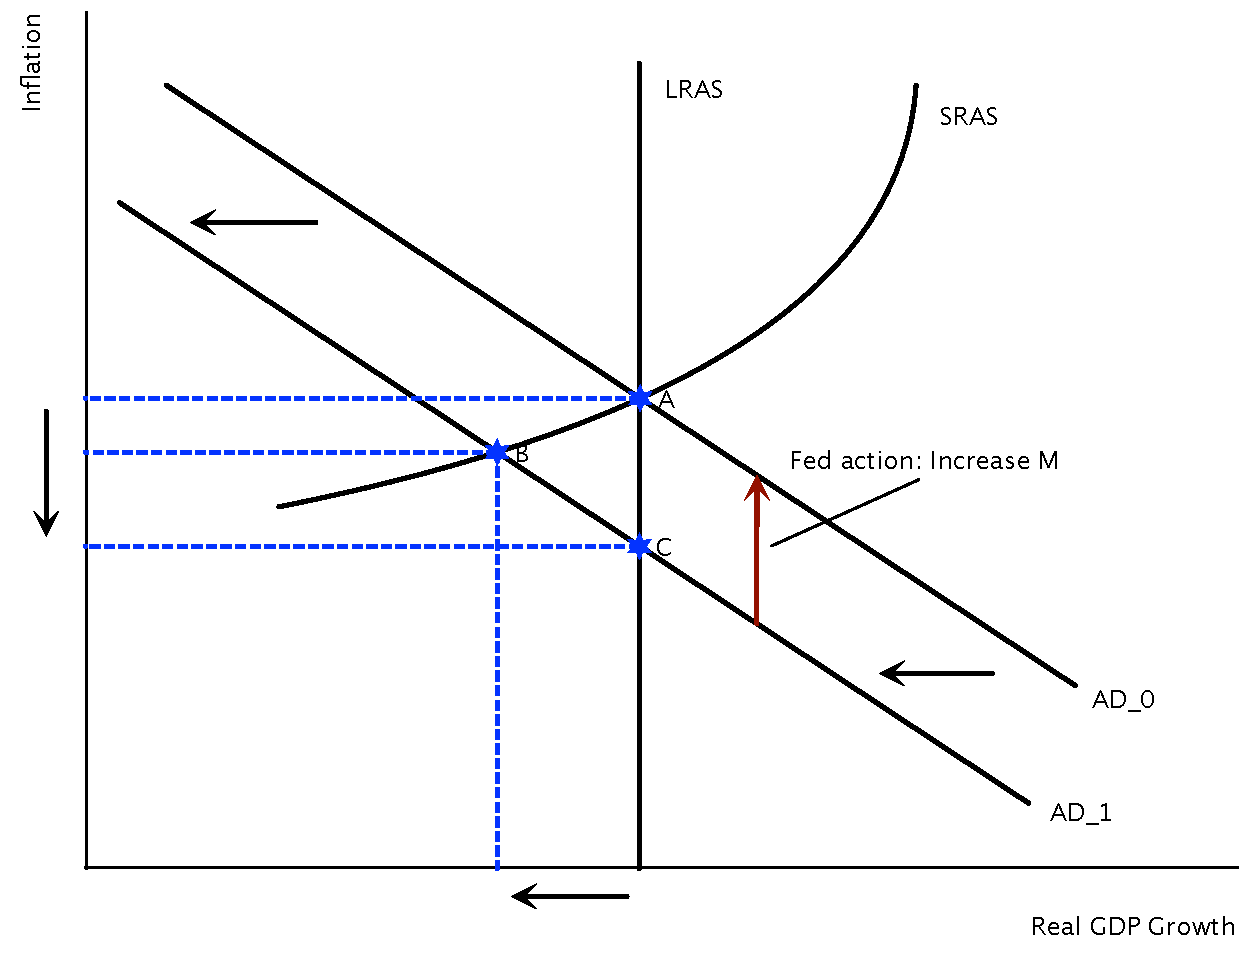
\includegraphics[scale=.40]{plot102.pdf}
	\caption{Monetary Policy}
\end{figure}
\end{frame}


\begin{frame}{Monetary Policy}
\begin{itemize}
\item Policies that attempt to pull an economy back from a recession are referred to as \dd{expansionary} policies, while those that attempt to slow down an ``overheated'' economy are \dd{contractionary} policies.


\end{itemize}
\end{frame}



\begin{frame}{Monetary Policy}
\begin{itemize}

	\item Issues with monetary policy:
	\begin{enumerate}
		\item Recognition lag: Time between start of recession and when policy is enacted.
		\item Imperfect control over the money supply: Don't know how much the money supply will increase in response to a higher monetary base.
		\item Exact impact of changes in $\vec{M}$ is not certain: Transmission mechanism: $\Delta \vec{M} \Rightarrow \Delta i \Rightarrow \Delta \vec{C}, \Delta \vec{I} \Rightarrow \Delta AD$.
		\item Effectiveness lag: Time it takes for changes in MS to affect AD.
	\end{enumerate}
	
	\item All these issues arise due to either the \dd{timing} or\dd{precision} of the policy.
	
\end{itemize}
\end{frame}


\begin{frame}{Monetary Policy}

\begin{itemize}
\item	Now, consider a real shock that causes the LRAS curve to shift left. How can the Fed combat decreasing real GDP?


\begin{figure}[H]
	\centering
	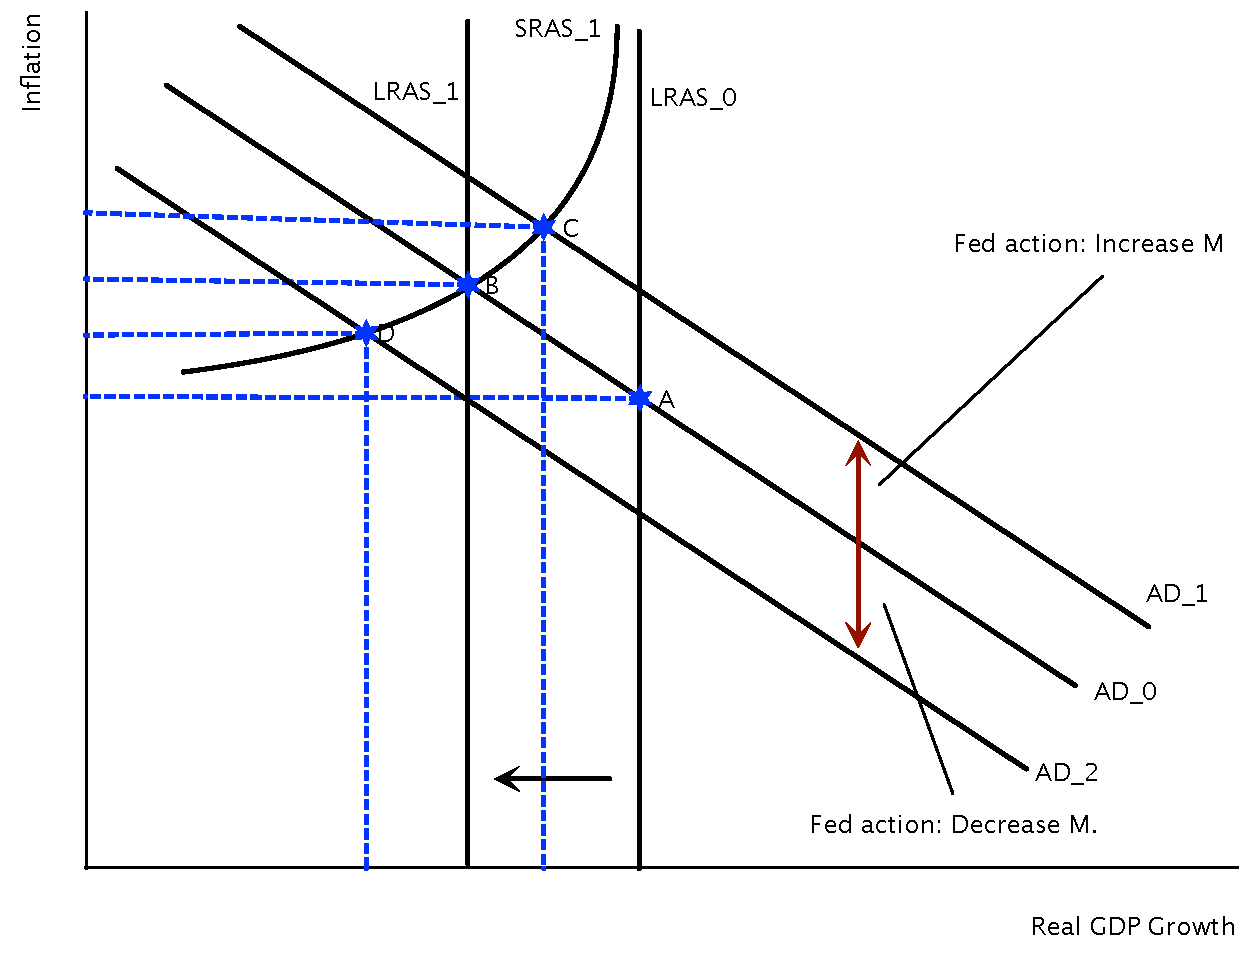
\includegraphics[scale=.35]{plot103.pdf}
	\caption{Negative Real Shock}
\end{figure}
\end{itemize}



\end{frame}

\begin{frame}{Monetary Policy}




\begin{itemize}
	\item When faced with a negative real shock, the Fed has to trade-off between too low a rate of GDP growth (and thus high unemployment) and too high a rate of inflation.
	\item \defn{Stagflation:} A stagnant economy (low/negative rates of output growth) with rising inflation.
\end{itemize}

\end{frame}

\section{Fiscal Policy}


\begin{frame}{Fiscal Policy}
\begin{itemize}
	\item An increase in government spending will shift AD to the \dd{right}, while a decrease in government spending will shift AD to the \dd{left}. 
	\item The government can finance increases in spending either through taxes or borrowing. In either case, fiscal policy is most effective when the economy is in a recession caused by low aggregate demand. 
	
	\item Importantly, the shift in AD will not perfectly respond to the change in government spending. 
\end{itemize}
\end{frame}

\begin{frame}{Fiscal Policy}
	\begin{itemize}
		
			\item Multiplier effect: Additional shifts in AD that result when expansionary fiscal policy increases incomes and thus spurs additional spending by consumers.
			
			\begin{figure}[H]
				\centering
				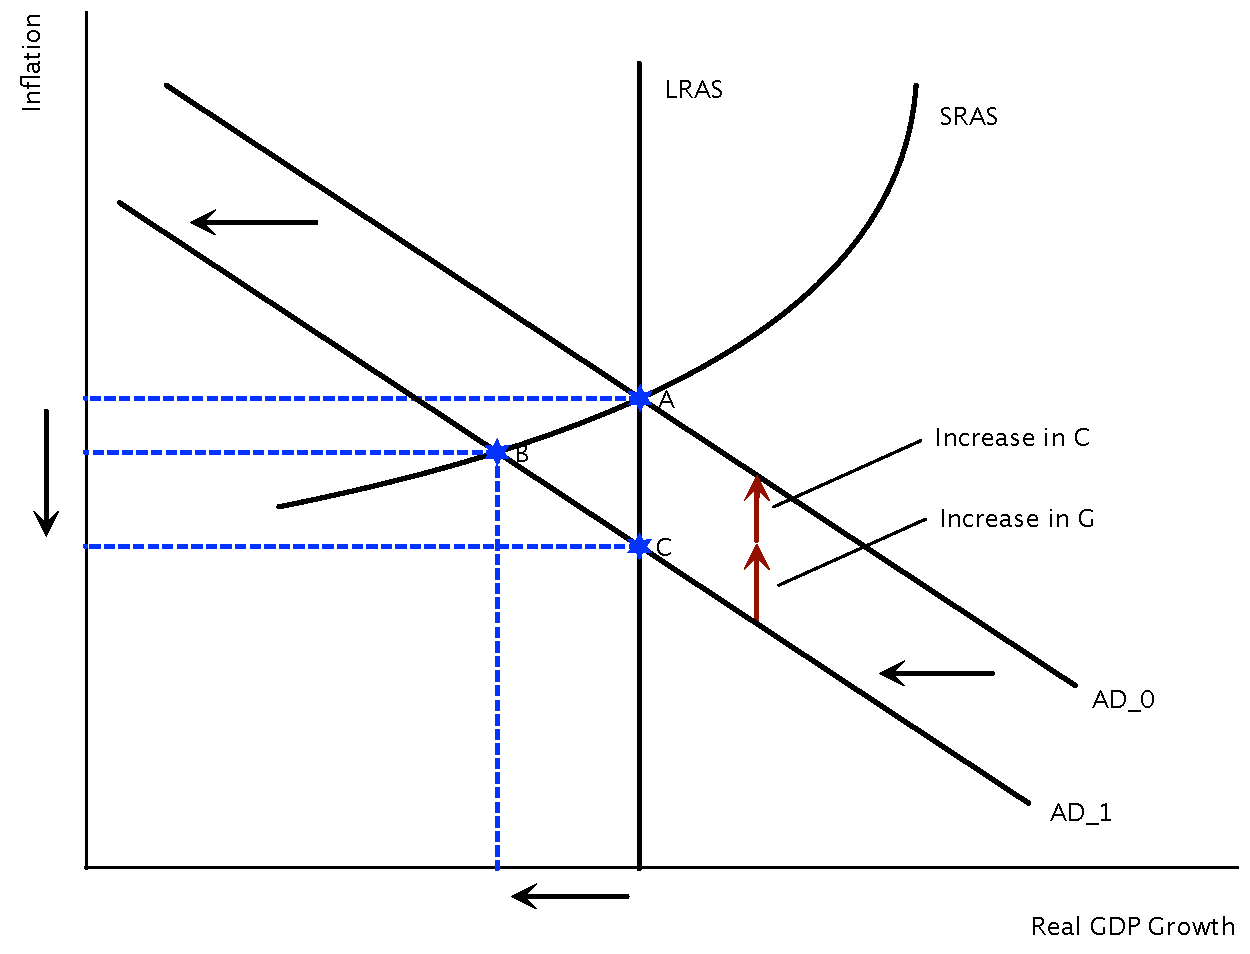
\includegraphics[scale=.35]{plot104.pdf}
				\caption{Multiplier Effect}
			\end{figure}
	\end{itemize}
\end{frame}

\begin{frame}{Fiscal Policy}
	\begin{itemize}
		
		\item Crowding out effect: The offset in AD that results when expansionary fiscal policy raises interest rates and thereby reduces private investment.
		
		
	\begin{figure}[H]
		\centering
		\caption{Crowding Out}
		\begin{subfigure}{.42\textwidth}
			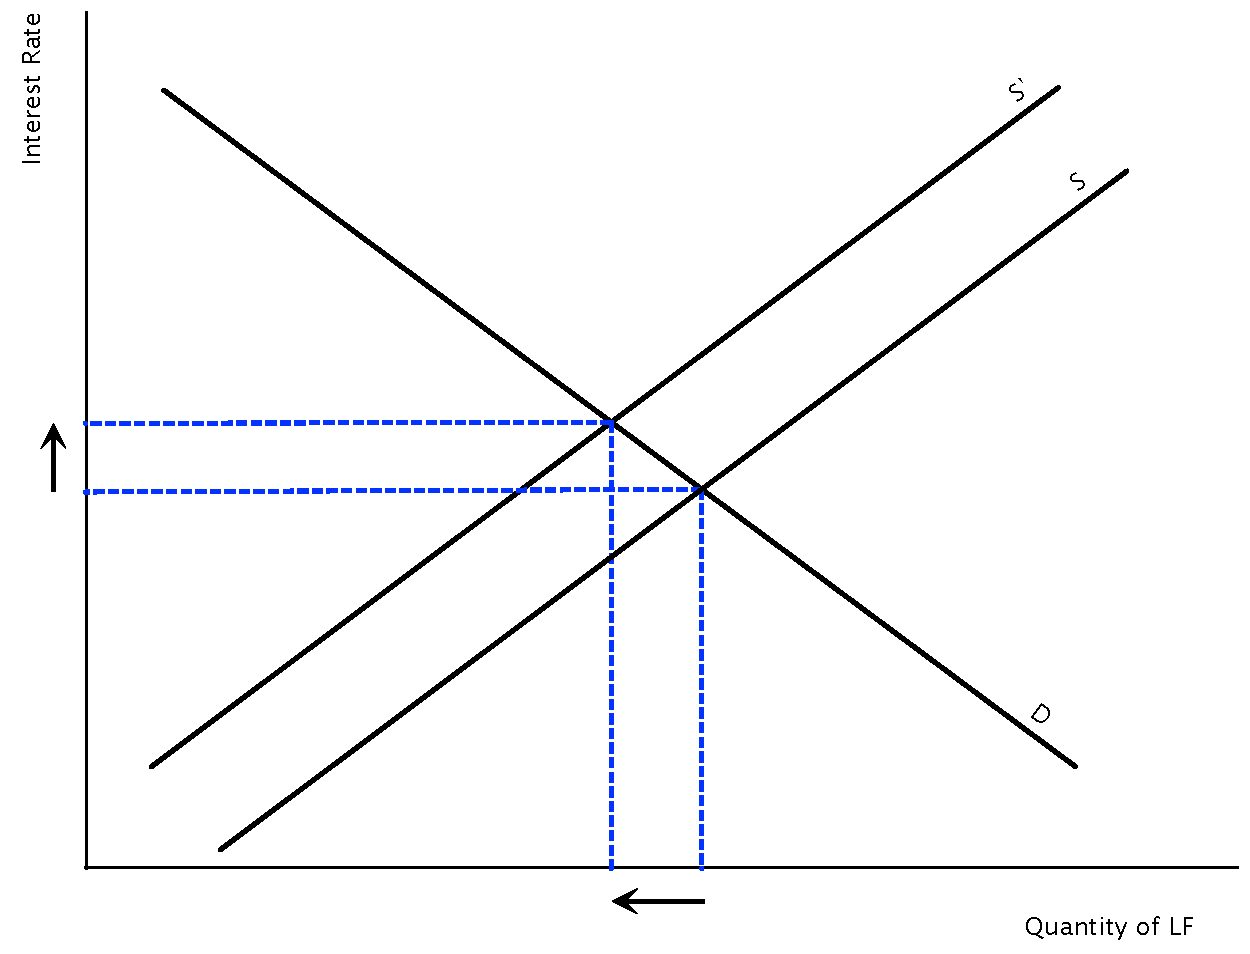
\includegraphics[scale=.25]{plot92.pdf}
			\caption{Market for Loanable Funds}
		\end{subfigure}%
		\begin{subfigure}{.42\textwidth}
			\centering
			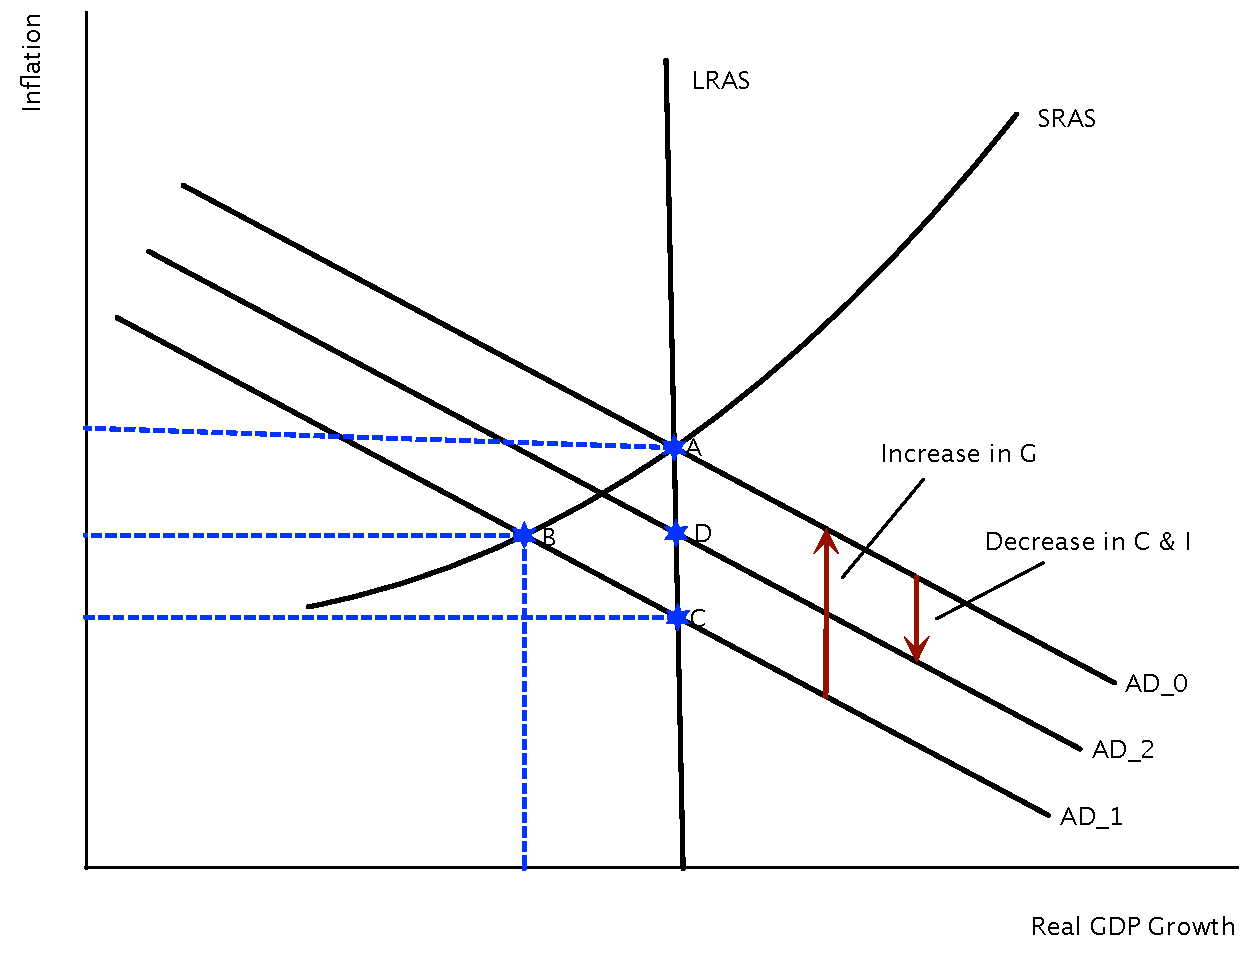
\includegraphics[scale=.25]{plot106.pdf}
			\caption{AS-AD Model}
		\end{subfigure}
	\end{figure}
	\end{itemize}
\end{frame}


\begin{frame}{Fiscal Policy}
	\begin{itemize}
		\item Another tool the government can use is changes in \dd{taxes}. Specifically, to spur spending the government would \dd{decrease} taxes and to decrease spending growth the government would \dd{increase} taxes.
		\item The size of the AD shift as a result of changing tax rates is also affected by the multiplier and crowding out effects, so the analysis is similar.
		\item Additionally, an important determinant of the size of the AD shift in response to tax change is the \dd{perceptions} of households about whether the tax change is \dd{permanent} or not.
	\end{itemize}
\end{frame}

\begin{frame}{Fiscal Policy}
	\begin{itemize}
		\item Issues with fiscal policy:
		\begin{enumerate}
			\item Crowding out limits effectiveness of fiscal policy.
			\item Difficult to spend enough money to have appreciable effect.
			\item Lags: recognition, legislative, implementation, and effectiveness.
		\end{enumerate}
		\item Because fiscal policy has a \dd{lag} between implementation and effectiveness, the efficacy of the policy as a tool to stabilize the economy in the short run is reduced.
		\item To avoid some of these potential lags, the government can implement \dd{automatic stabilizers}: changes in fiscal policy that stimulate AD in a recession without the need for explicit action by policymakers
	\end{itemize}
\end{frame}

\begin{frame}{Readings and Assignments}
\begin{itemize}
	\item Today: Mankiw Ch. 34
	\item Next time: \frownie{} \frownie{} \frownie{}
	\item Problem Set 6, section 4
\end{itemize}
\end{frame}

\end{document}